\documentclass{article}

\usepackage{enumerate}
\usepackage{graphicx}
\usepackage{hyperref}
\usepackage[shortlabels]{enumitem}
\usepackage{subcaption}
\usepackage{svg}
\usepackage[disable]{todonotes}
% \usepackage{todonotes}
\usepackage{url}

\title{Research topics\\Fixed-viewpoint procedural generation of digital nature landscapes.}
\author{Lars van Arkel}

\begin{document}
 
\maketitle

\section{Introduction}
Procedural Content Generation (PCG) has been actively researched in computer graphics for years. For developers generating virtual content can become time-intensive, and PCG has been used to reduce the workload of creating virtual terrains. One important aspect is the trade-off between the control the user has over the generated terrain against the amount of effort required to create the terrain. For this research, we will be designing a system to generate complete landscapes which will be rendered from ground level. Besides combining multiple features, this research will aim to give a qualitative evaluation of the generated terrain with rules that can be specified by the designer. This system will then be used to create landscapes as part of the Growing Roots research project.

\section{Problem statement}
As part of the Growing Roots research project \footnote{Growing Roots. From \url{https://growingroots.nl}, retrieved at 16-11-2023}, a device called the ``virtual window" is developed by the company TexTown Games. \footnote{Design2Connect - TexTown Games. From \url{https://textowngames.nl/portfolio/design2connect/}, retrieved at 11-16-2023}. This device tracks the position of a person in front of a monitor and projects a landscape on the screen based on where the person is standing. Currently, only handcrafted landscapes are used for testing the system. For further research related to emotional impressions of landscapes, more environments are needed that differ in visually distinguishable parameters, such as the density of trees or the color and types of vegetation used. Handcrafting landscapes takes a significant amount of time, so the ability to create more terrains automatically is required. The landscapes generated will be landscapes of nature, with some man-made structures such as roads or benches. 

The generated terrain will only be used for the virtual window, which means that the camera will not move around the landscape. This limits the size and amount of terrain that needs to be generated. Therefore, each feature's order and properties will be generated with this rule in consideration.

As further research will focus on the effect of different terrain features, the researcher needs control over the terrain they want to create. This control should allow the user to select broader features of the terrain, such as the kind of ecology the terrain represents, and finer features, such as the density of vegetation or ruggedness of the ground.

As the system will be used by people who are not necessarily designers or programmers, the generation of the terrain will be automated with little user input. Because of this, we must be able to verify whether the generated terrain adheres to required constraints. These features can be broad for the entire terrain, such as that some desired biomes are included, or specific to the point of view, such that a large part of the generated is visible from the viewpoint.

\section{Research questions}
\begin{enumerate}[label={RQ \arabic*:}]
    \item How can we generate each component in a landscape, and how do these components work together and interact to create a landscape suited for a single point of view?
    \begin{enumerate}[label={RQ 1.\arabic*:}]
        \item What components are required to generate a landscape?
        \item How can we generate each component required for the landscape?
        \item How can we connect all components to create a landscape for a single point of view?
    \end{enumerate}

    \item How can we parameterise each component to create distinctive environments, while the effect of each parameter is clear?
    \begin{enumerate}[label={RQ 2.\arabic*:}]
        \item How do we define different environments to be distinctive?
        \item How can we use parameters to distinguish between different environments?
    \end{enumerate}

    \item In what ways can we validate the procedurally generated terrain?
    \begin{enumerate}[label={RQ 3.\arabic*:}]
        \item How can different requirements be translated into rules to validate the terrain?
        \item How can the terrain generation be influenced by the validation to create terrain conforming to certain rules?
    \end{enumerate}
\end{enumerate}

\section{Approach}
The proposed research questions will be answered with multiple steps. Firstly, the requirements of the system, as defined by RQ 1.1, 2.1 and 3.1, will be gathered from researchers involved with the Growing Roots project and the developers of TexTown Games, as well as related research on Digital nature. With this, we establish a scope for a small prototype to answer the research questions.

For each of the research questions, the first sub-question is related to finding the requirements of the research question. These sub-questions will be answered in several ways. First, related research into procedural generation, digital nature and the Growing Roots research project will be analysed to find relevant topics. Additionally, brainstorming sessions with related stakeholders will refine the previously found requirements. These stakeholders consist of researchers part of the Growing Roots project, which will continue the research, and employees of TexTown Games involved with the project.

For RQ 1.2, we can use the background literature for each of the required features to select an approach of generating each component individually. An implementation of this will be included in the prototype.

When all requirements are gathered, an architecture of the system will be created that shows how the proposed system works. This architecture contains the interaction between different components (RQ 1.3), a connection between high-level features from a designer and the low-level features used by each component (RQ 2.2), as well as how validation techniques are used in landscape generation (RQ 3.2).

From this architecture, a prototype will be created. Due to the technology already used by TexTown Games, this prototype will be created using the Unity game engine and C\# scripts \footnote{Unity Real-Time development platform, from \url{https://unity.com}}. To create landscapes, assets such as textures and models of vegetation, trees and man-made objects will be provided and the generation of these is not part of this research.

%RQ 1.1 Brainstorm with researcher / company. Look at related research
%RQ 1.2 Look at related research. Build prototype components for each individual component.
%RQ 1.3 Define requirements for a landscape for a single point of view. Create an architecture to connect components.

%RQ 2.1 Create requirements for different environments (tended/wild, open/closed, biomes) with researcher / company / background research.
%RQ 2.2 Connect generation parameters to requirements. Adapt architecture to support parameters.

%RQ 3.1 Brainstorm with researcher / TTG. In the brainstorm, find the usefulness of validating the requirements to future research.
%RQ 3.2 Add validation to architecture. Decide how validation will be used to influence terrain generation

\section{Background}
The generation of a virtual terrain can be split up in multiple components which are connected to create a complete landscape. Firstly, the terrain itself needs to be created, after which other components are generated that interact with the terrain to create the complete terrain. The following sections describe prior research and techniques for generating individual components, as well as different ways that are proposed to connect these components.

\subsection{Generation of terrain}
The topic of procedural terrain generation has been researched for multiple decades. A 2-dimensional height map, represented as a grayscale image, is the most common technique for generating terrain. When converting this height map to a 3-dimensional terrain, a 3D plane uses the height map to scale each vertex of the terrain to a specified height. This approach is widely used due to its simplicity but has some downsides. Because the height map is projected onto the plane, the terrain cannot have multiple sections of terrain overlapping each other, such as overhangs or caves. Although some solutions allow for overhangs \cite{gamito_procedural_2003}, they usually require solutions tailored to the desired terrain.

Alternatively, the terrain can be generated using a volumetric data structure, such as a 3-dimensional grid \cite{dey_procedural_2018}. With this approach, the generated terrain depends on whether the volumes of each location in the grid are filled. The most famous example that uses a voxel-based terrain is the video game Minecraft \footnote{Minecraft. From \url{https://minecraft.net}, retrieved on 28-11-2023}, which uses voxels to create a crude, blocky terrain. Fine-grained terrains can also be transformed into smooth terrain using techniques such as the surface nets method \cite{gibson_constrained_1998}. Although this approach allows for complex structures including caves \cite{cui_voxel-based_2011} and overhangs, the limitation of this approach is the larger storage size of all data.

The following sections will focus on generating specific parts of a landscape, focusing mainly on techniques using height maps instead of volumetric data structures. These sections provide insight into how specific parts of the landscape are generated.

\subsubsection{Fractal terrain} \todo{Images}
A popular approach to generate procedural terrain is to use fractals. In this approach, a terrain function is evaluated on multiple scales to generate terrain that has large-scale features but is also detailed on a lower scale \cite{shaker_procedural_2016}. One way to create such terrain is to use noise functions such as Perlin noise \cite{musgrave_synthesis_1989}, where the function is evaluated on multiple frequencies and summed to get the total height of the terrain. Because the noise is calculated on multiple frequencies, the terrain becomes less smooth, and both the large-scale terrain, as well as details, are created. 
Because noise functions only depend on the input coordinates, these algorithms can be applied easily to GPU-based implementations \cite{schneider_real-time_2006}. \todo{Show generated noise images}

Instead of noise functions, a midpoint displacement algorithm is another way to generate terrain. With this algorithm, a triangle or grid gets subdivided into smaller primitives, and the height of each midpoint is updated with a random value. This value grows smaller with each iteration, resulting in small changes in local areas, and large changes in global areas \cite{sala_mathematics_2002}. One type of midpoint displacement algorithm, the diamond-square algorithm recursively subdivides a grid of points to approximate Fractal Brownian motion \cite{miller_definition_1986}. This algorithm is visualised in figure \ref{fig:diamond_square}

\begin{figure}
    \centering
    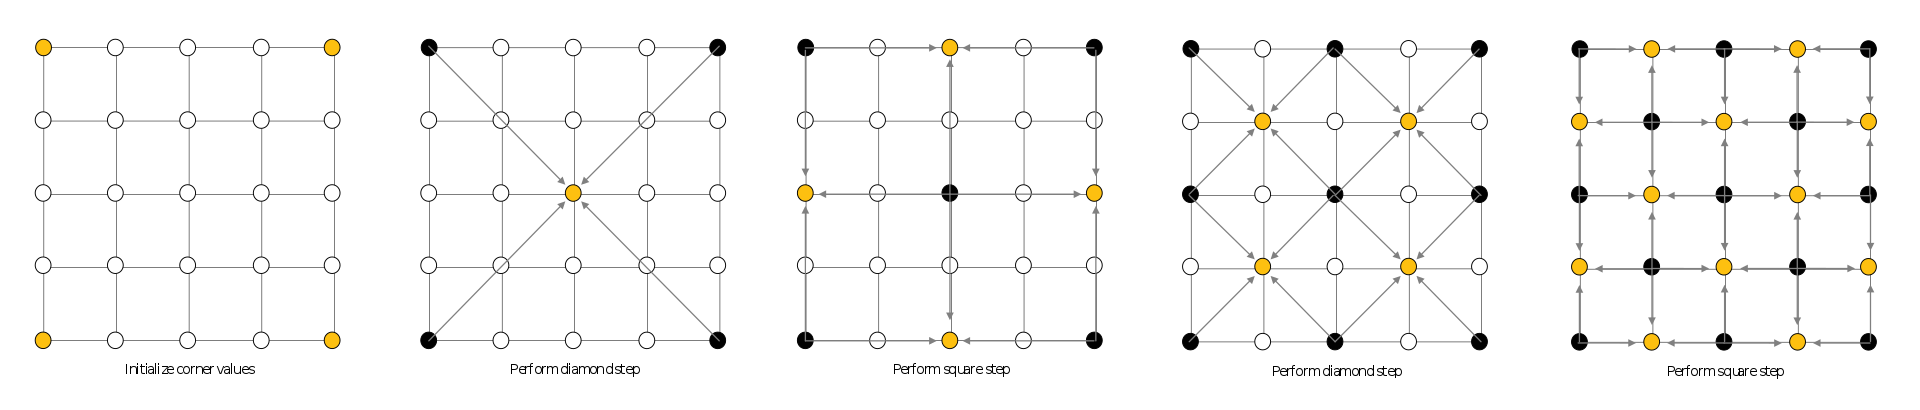
\includegraphics[width=\textwidth]{figures/Diamond_Square}
    \caption{Two iterations of the diamond-square algorithm. The yellow dots represent the vertices manipulated in each operation, and the black dots represent the values used in interpolation\protect\footnotemark.}
    \label{fig:diamond_square}
\end{figure}

\footnotetext{By Christopher Ewin - Own work. Retrieved from \url{https://commons.wikimedia.org/w/index.php?curid=42510593}}

Instead of using a single approach, the combination of multiple functions, such as adding Voronoi noise to a midpoint displacement map, can also result in different types of terrains \cite{olsen_realtime_2004}.

\subsubsection{Erosion algorithms}
Although using fractal terrain works well to generate terrains, the self-similar nature of the techniques used does not result in realistic-looking terrain. Because of this, physical simulation is often used to approximate more realistic terrain. Most techniques follow processes that resemble erosion, which are divided into hydraulic erosion and thermal weathering \cite{musgrave_synthesis_1989}. These types of simulation are mainly used to enhance the quality of a terrain generated by fractal brownian motion, instead of being used to fully generate a terrain.

Hydraulic erosion models the use of water to transport sediment from higher locations to lower locations. This can be used in conjunction with rivers, or by simulating rainfall and water transport. There are several techniques for this simulation, implemented on both the CPU and GPU \cite{benes_visual_2002} \cite{stava_interactive_2008}. Hydraulic erosion works by discretizing the surface, where each chunk contains the height of the terrain, as well as the amount of water contained in the chunk. Updating the state of the simulation is done using Cellular automata, with each iteration interchanging water and sediment between neighbours \cite{dambrosio_cellular_2001}. An example of a step in this algorithm can be seen in figure \ref{fig:hydraulic-erosion}.

\begin{figure}
    \centering
    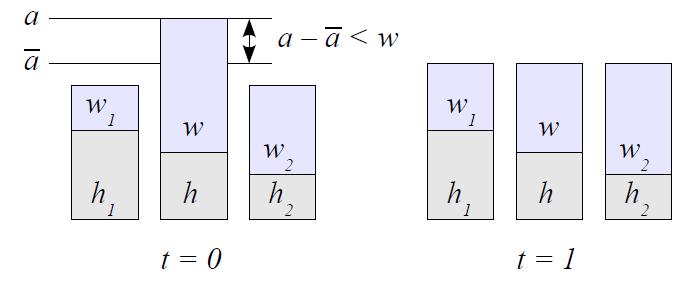
\includegraphics[width=\textwidth]{figures/Hydraulic_erosion.PNG}
    \caption{An example of water transport in a hydraulic erosion simulation, from \cite{olsen_realtime_2004}.}
    \label{fig:hydraulic-erosion}
\end{figure}



Thermal erosion describes the way that material is eroded by several processes that break down the terrain, from which the material moves down a slope to accumulate at the bottom \cite{musgrave_synthesis_1989}. Similar to hydraulic erosion, it works by using cellular automata to transport soil to neighbouring locations. Instead of using water, the difference in height of neighbours is compared, and if it exceeds a threshold a portion of the terrain is moved to the lower level.

\subsubsection{Agent-based algorithms}
The previous algorithms manipulate the terrain as a whole. Another option would be to use software agents to manipulate the terrain on a local scale. In their paper \cite{doran_controlled_2010}, Doran and Parberry have used multiple types of software agents that create coastlines, mountains and rivers. Each agent has a location on the map and perceives their direct environment. They can modify the terrain using a directive, such as generating a coastline that connects two randomly generated points or creating a river connecting the top of a mountain and the coast. In more recent work, software agents were expanded to offer more control to the designer \cite{skold_generating_2023}. In other work, software agents were used to generate a road network and place buildings to form a city \cite{lechner_procedural_2003}.

\subsubsection{Rivers}
On a terrain, the generation of rivers is directly related to the landscape itself. Rivers have the requirement to be placed in a landscape, such as that the direction of the river should move along a flat part of terrain, or move downwards.

One way of generating rivers is to generate rivers and elevation at the same time. Belhadj and Audibert \cite{belhadj_modeling_2005} generate a network of rivers and ridges, and use this combined with a modified midpoint displacement algorithm to generate the rest of the terrain. After ridges are randomly generated, points are placed on ridges and simulate gravity to roll down the slope. With this approach, rivers show realistic behaviour connected to the elevation of the ridges.

If the terrain consists of both mountains and coastlines, a river can also be generated by finding a random point on the coast and a random point on the mountain, and generating a random path between these points \cite{doran_controlled_2010} \cite{prusinkiewicz_fractal_1993}.

Alternatively, rivers can be generated by placing several control points on the map and interpolating between these control points to generate a path \cite{smelik_declarative_2011}. To fill the path of the river with a mesh, a 2D cross-section can be used to extrapolate a shape for the entire path \cite{huijser_procedural_2010}. In this paper, the cross-section is also used to add vegetation and textures to the river.

% Water by Y-level

% Realtime library
% Declarative approach
% New papers added to tablet

% Masks / moisture maps (Zero dawn)
% Rain/erosion simuation (Realistic modeling and rendering of plant ecosystems)


\subsubsection{Texturing}
To create a terrain, adding textures is vital in making the terrain realistic. One approach is to create textures beforehand for different types of terrain and to blend these textures depending on factors such as the height and steepness of the terrain \cite{schneider_real-time_2006} \cite{kahoun_realtime_2013}. With this approach, areas near water use textures that represent beaches such as sand, while steep peaks use a stone texture. Additionally, the texture can be defined by the ecosystem the terrain is part of \cite{hammes_modeling_2001}. Edges between ecosystems can be generated by blending different types of textures.

\subsection{Placement of vegetation}
When generating a landscape representing nature, an important step is placing vegetation in ways that are realistic and visually appealing. Adding vegetation to a landscape consists of different kinds of elements, from small vegetation such as grass and small bushes to large structures such as trees. The following sections describe multiple ways of placing and distributing vegetation.

\subsubsection{Distributed placement}
An easy way to place vegetation is by planting each plant randomly. As each plant or tree is a physical object, plants cannot be placed too close to each other or they would overlap.

\begin{figure}
    \begin{subfigure}[h]{0.5\linewidth}
        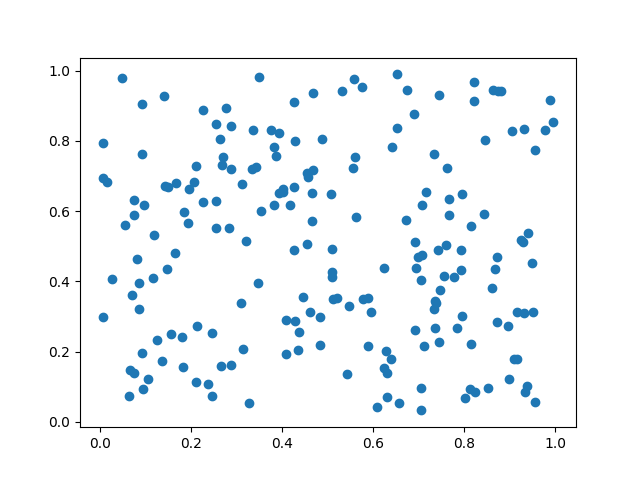
\includegraphics[width=\linewidth]{figures/distribution_random.png}
        \caption{Random distribution}
    \end{subfigure}
    \begin{subfigure}[h]{0.5\linewidth}
        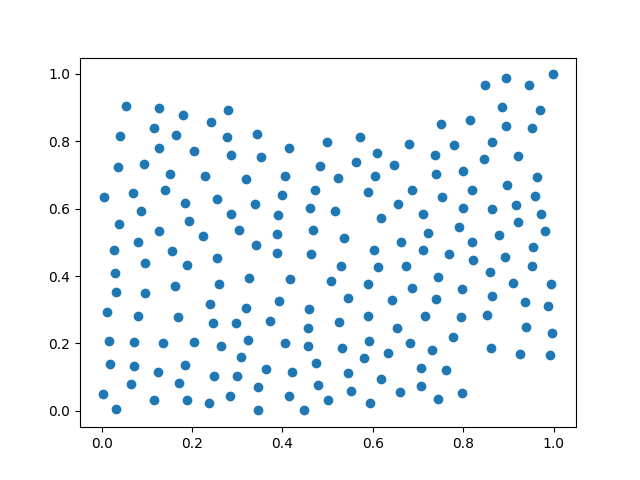
\includegraphics[width=\linewidth]{figures/distribution_pdd.png}
        \caption{PDD distribution}
    \end{subfigure}
    \caption{Comparison of Random and Poisson Disk Distributions for 200 samples}
    \label{fig:random-distributions}
\end{figure}

One way to solve this is to specify a boundary radius and place plants randomly in locations where the closest plant is further away than that distance. Although this works, Casey Muratori showed in a blog post that this naive approach is inefficient when the density of plants increases \cite{muratori_color_2014}. A more efficient way to generate random positions is to use Poisson Distribution Disks (PDDs). A Poisson distribution disk allows patterns to be generated where each point has a minimal separation, as shown in figure \ref{fig:random-distributions}. Efficient algorithms use Voronoi diagrams to create these patterns with a time complexity of $O(N \log{} N)$ \cite{jones_efficient_2006}. Another implementation, based on fluid simulations, uses a smoothing kernel which moves an initial set of points so that the standard deviation of the distances between points is lowered \cite{jiang_blue_2015}.

Another way of distributing points is to have an initial set of points, for instance, points on a grid, and to randomly move each point around its initial location. Although simple, this technique has been used to create points that look seemingly random \cite{hammes_modeling_2001} \cite{van_muijden_gpu-based_2017}.

\subsubsection{Tiling}
Instead of randomly generating positions for the entirety of the terrain, another approach would be to tile smaller point distributions on a larger field. Instead of repeating a single tile repeatedly, Wang tiles can be used instead \cite{cohen_wang_2003}. Wang tiles are tiles with coloured edges, and each coloured edge can be connected with edges of the same colour. This tiling algorithm results in an aperiodic layout which removes the repetition from using the same point distribution multiple times.

\subsubsection{Ecosystem simulation} \label{sec:background/ecosystemsim}
Another way to place vegetation is to perform an ecosystem simulation. This technique simulates the growth of plants, as well as the competition for resources. It uses L-systems to grow plants based on the self-thinning phenomenon \cite{deussen_realistic_1998} \cite{lane_generating_2002}. This suggests that when the density of plants is low, all plants grow without competition. When the population has reached a certain density, plants need to compete for resources, and larger plants dominate smaller, weaker plants. Using this type of simulation can be done on a single type of plant, or on multiple different kinds of plants of a similar type, such as different kinds of trees or grass.

% Poisson distribution disks: 
%       GPU-Based Real-Time Procedural Distribution of Vegetation on Large-Scale Virtual Terrains
%       Generating and Rendering Large Scale Tiled Plant Populations
%       Blue Noise Sampling using an SPH–based Method (Background)

% Random jitter on grid
%       Modeling of Ecosystems as a Data Source for Real-Time Terrain Rendering
%       GPU-based procedural placement in Horizon Zero Dawn

% Wang tiles
%       Generating and Rendering Large Scale Tiled Plant Populations
%       Terrain Guided Multi-Level Instancing of Highly Complex Plant Populations

% Dithering
%       GPU-based procedural placement in Horizon Zero Dawn
%       Realistic modeling and rendering of plant ecosystems (Initializes)



% Generating Spatial Distributions for Multilevel Models of Plant Communities (Simulates with grammars)
% Procedural Generation and Rendering of Realistic, Navigable Forest Environments: An Open-Source Tool
% Realistic modeling and rendering of plant ecosystems


\subsubsection{Blending environments}
To add variety to the generated landscape, adding different types of terrain might be valuable. An example is the edge of a forest, where one section of the terrain consists of grassland, and the rest is the forest. In ecology, the concept of biomes has been established to categorise different types of terrain. Using metrics such as average temperature or the amount of precipitation allows different environments to be categorised. Two popular ways of categorising biomes are those from Holdridge and Whittaker \cite{mucina_biome_2019}. Holdridge's scheme, developed in 1947, uses three metrics; average temperature, precipitation and evapotranspiration, the process that moves water into the atmosphere by evaporating from the ground, or transpiration from trees and vegetation. The system of Whittaker, proposed in 1970, uses only the average temperature and precipitation to categorise different biomes. The two schemes can be seen in figure \ref{fig:biome_schemes}.

\begin{figure}
    \centering
    \begin{subfigure}{0.45\linewidth}
        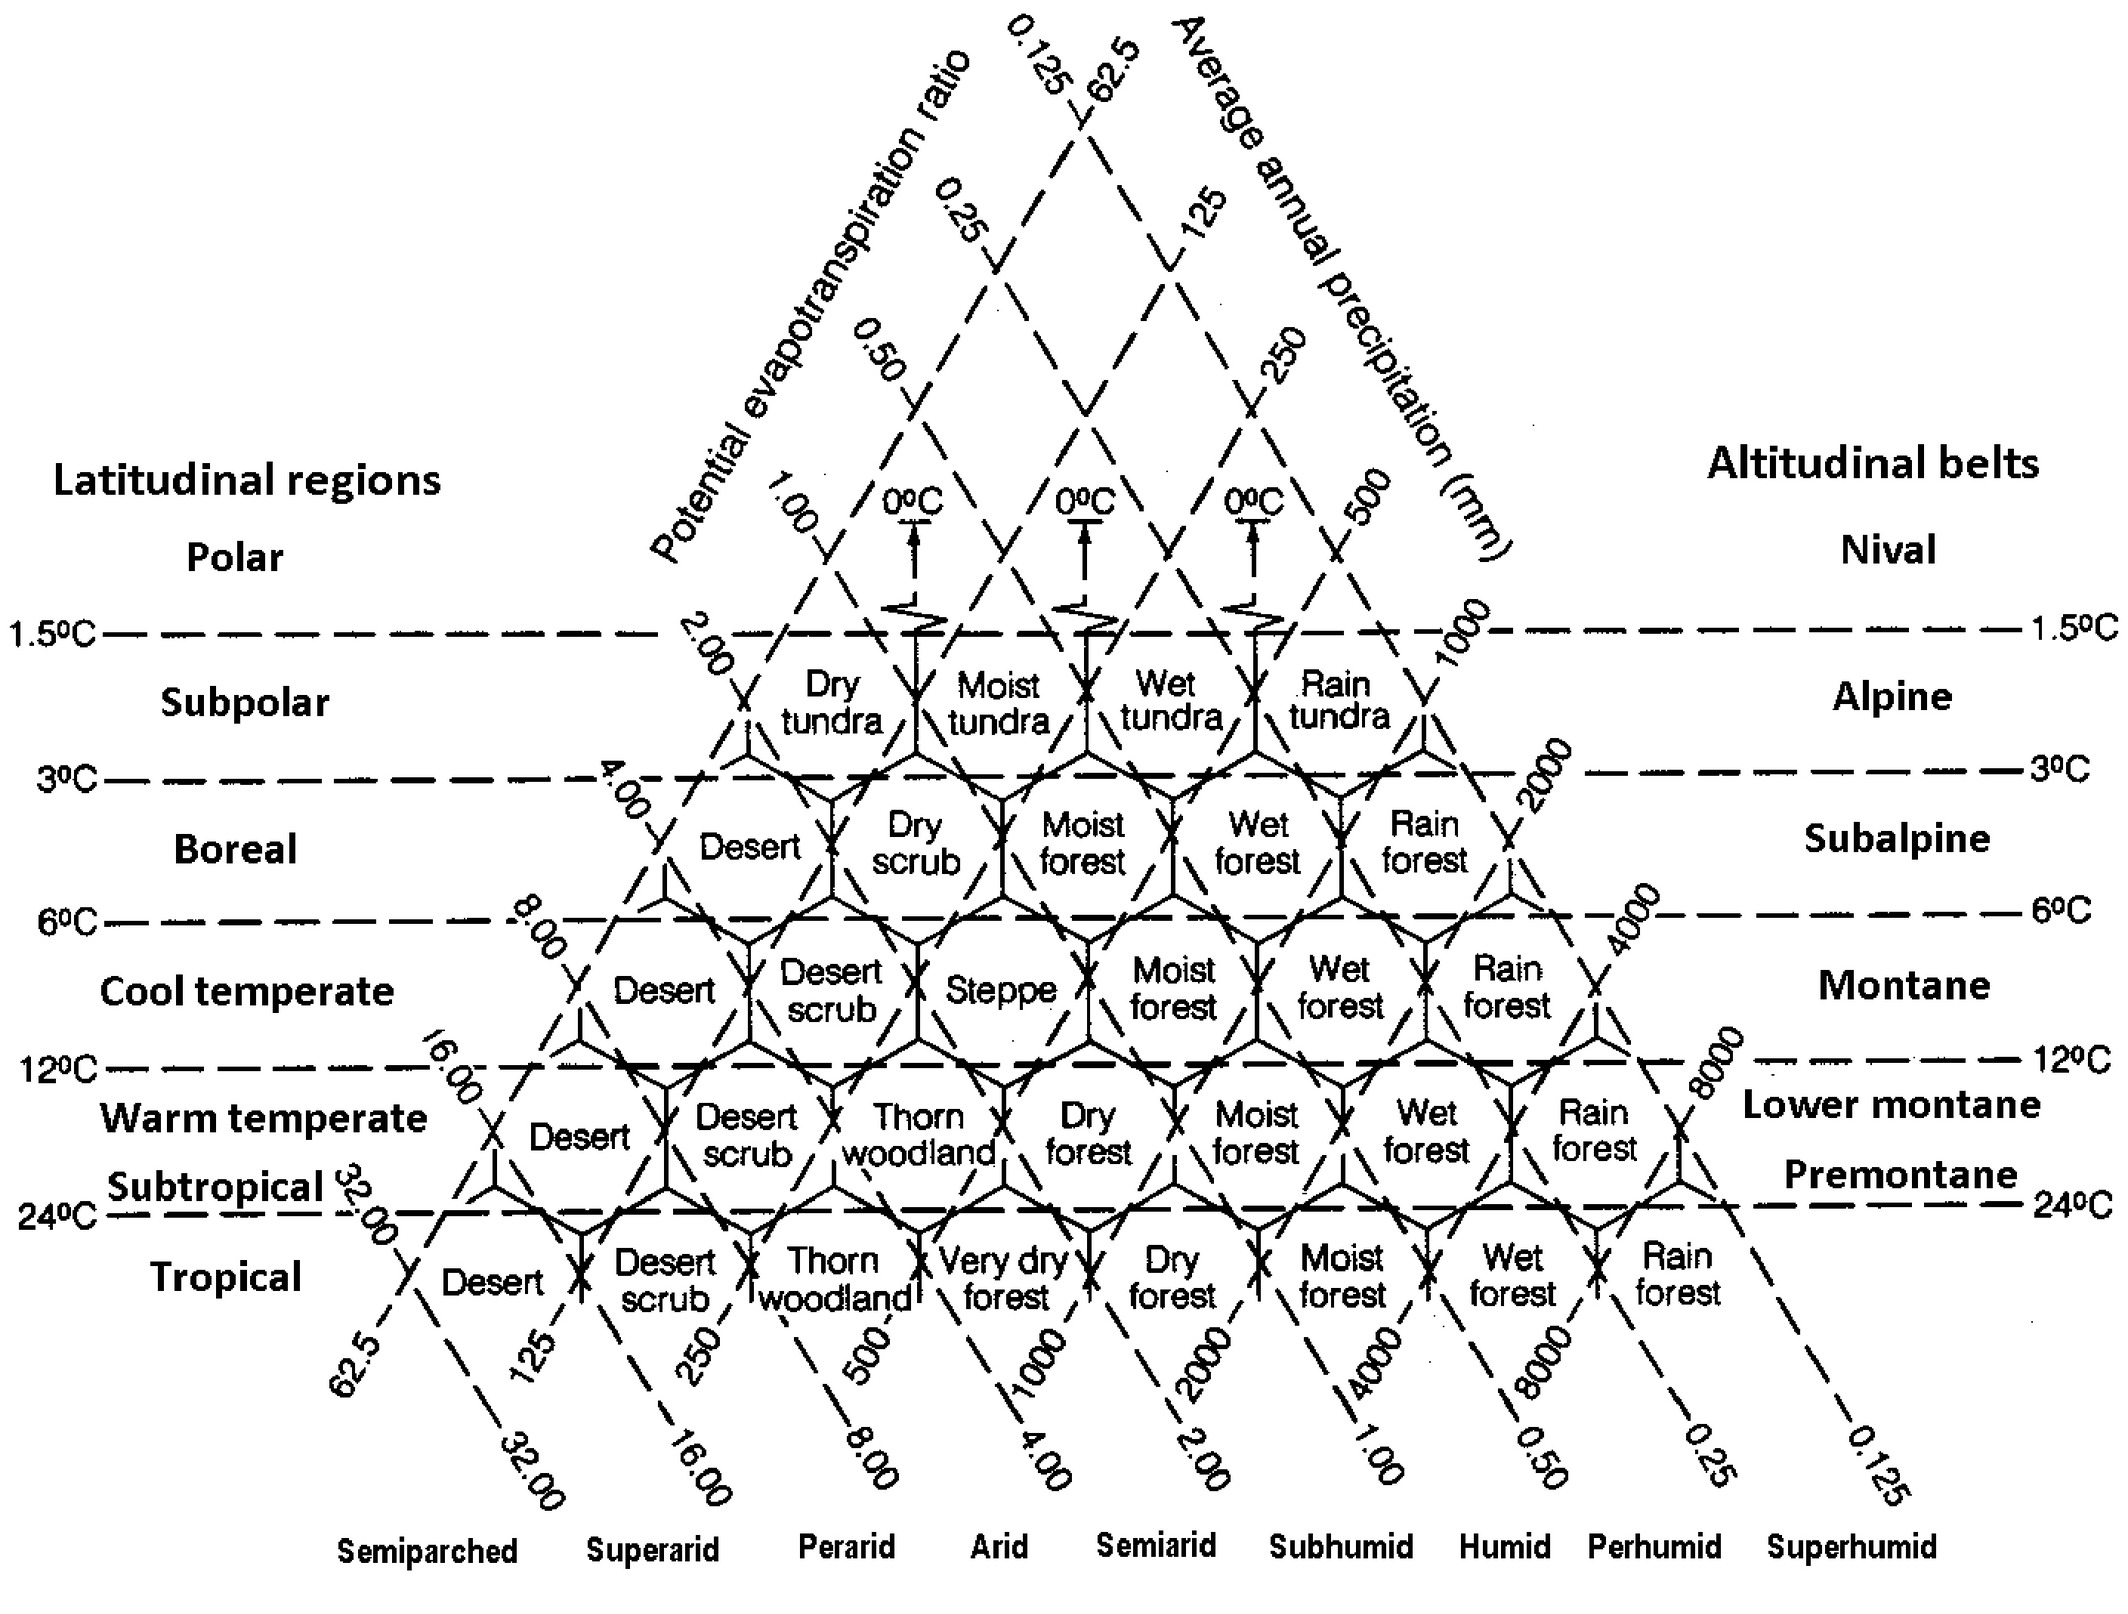
\includegraphics[width=\linewidth]{figures/biome_holdridge.png}
        \caption{Model of biomes proposed by Holdridge.}
        \label{fig:biome_holdridge}
    \end{subfigure}
    \hfill
    \begin{subfigure}{0.45\linewidth}
        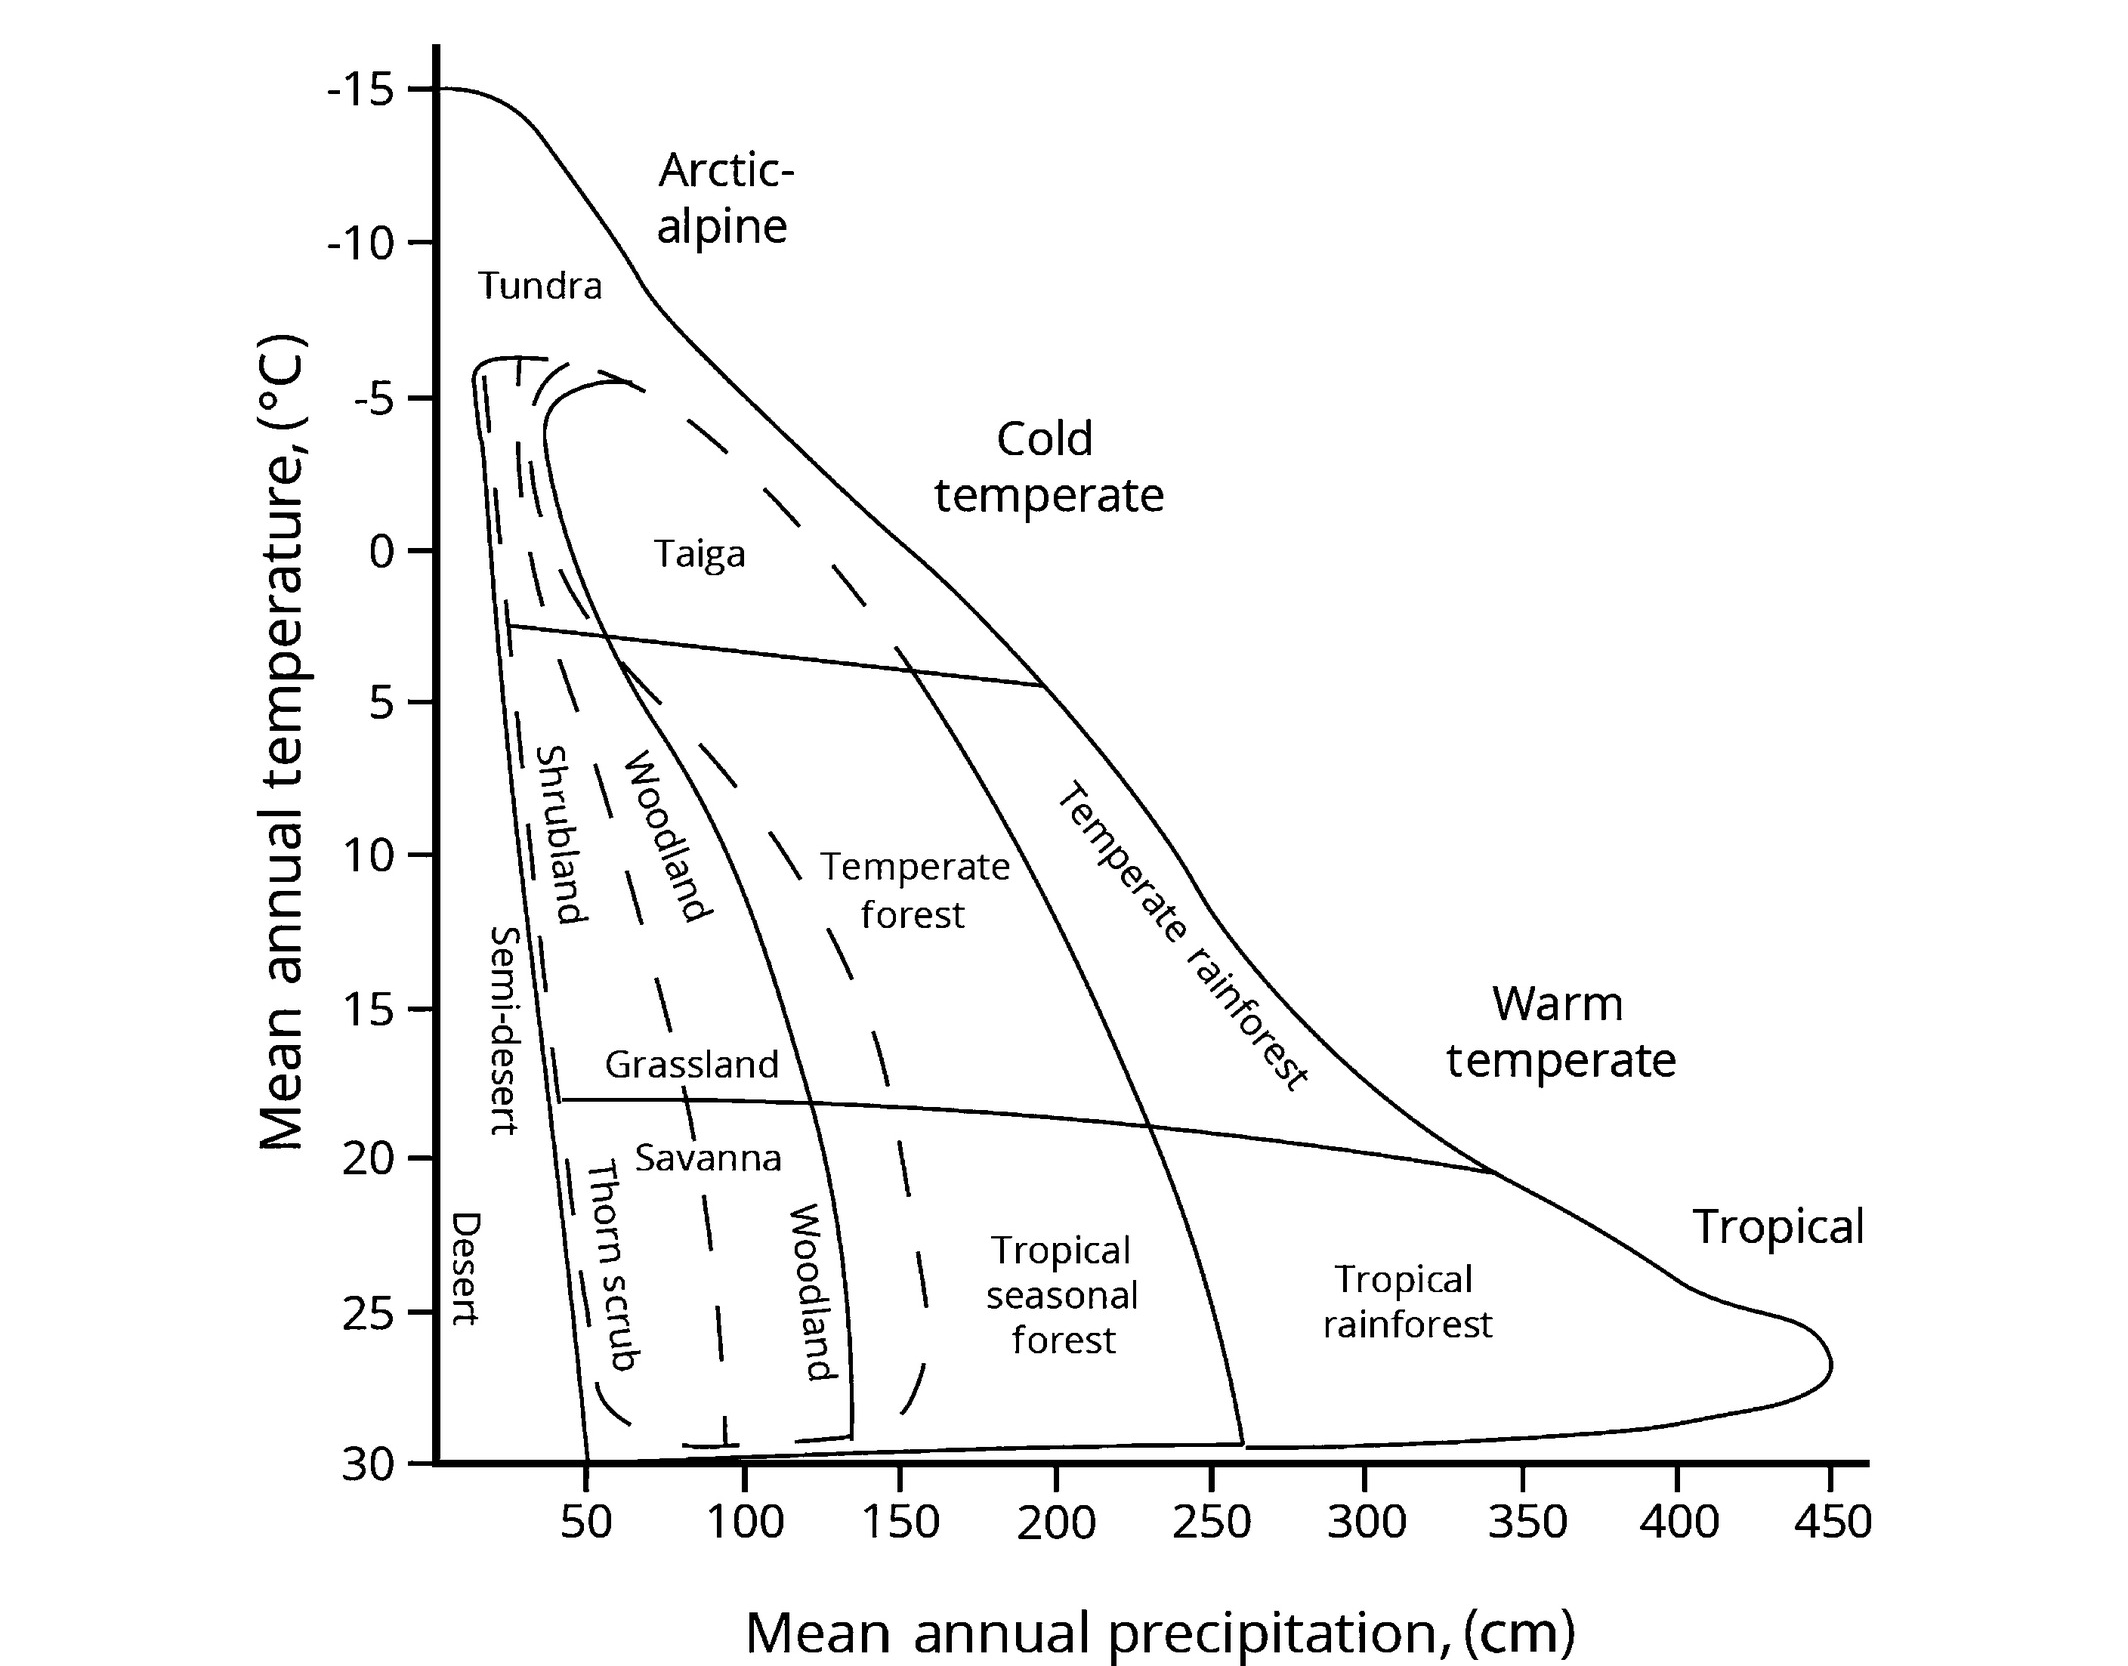
\includegraphics[width=\linewidth]{figures/biome_whittaker.png}
        \caption{Model of biomes proposed by Whittaker.}
        \label{fig:biome_whittaker}
    \end{subfigure}

    \caption{Two classification models of biomes, retrieved from \cite{mucina_biome_2019}.}
    \label{fig:biome_schemes}
\end{figure}

In the previous example, the biome was determined by climate parameters. The type of environment can also be established by using other procedurally generated data. For instance, the terrain itself can also provide information on what the terrain should look like \cite{hammes_modeling_2001}, such as the slope, elevation and humidity of the terrain. Additionally, the presence and rivers and the overall humidity of the ground can influence the terrain generated \cite{do_nascimento_gpu-based_2018} \cite{van_muijden_gpu-based_2017}. In these examples, each type of plant or tree has a preferred range of parameters in which it will be generated.

\subsection{Connecting components}
The previous sections have elaborated on different components used in procedural terrain generation. To generate terrain that resembles a landscape, these features must be combined. The following section describes different ways that these components can be connected, and how the requirements of each component interact with other components.

\subsubsection{Level of detail}
When placing vegetation, there is a difference between placing large trees and smaller bushes and grass. Trees are larger and the branches prevent other trees from being placed too close to each other. For bushes and grass, this is much smaller, and they can also grow under the branches. In their paper, Hammes defines eight different layers that each cover a different type of vegetation on a different scale \cite{hammes_modeling_2001}. For a large scene, this can be used as a level of detail to reduce the complexity of areas that are further away and to increase the detail for closer sections of terrain. To resolve placement conflicts between layers, do Nascimento added a function to calculate the zone of influence of objects on a higher layer, which acts as a probability mask for objects on a lower layer \cite{do_nascimento_gpu-based_2018}.

\subsubsection{Probabilities and masking}
When placing vegetation on a terrain, it cannot be placed on certain areas. For instance in water, or on slopes that are too steep. There have been multiple ways to resolve these issues. When categorising the terrain into ecotypes, as done by Hammes \cite{hammes_modeling_2001}, parts of the terrain that are unsuited for vegetation simply will not include any vegetation at all. Alternatively, Olsen assigns placement scores based on flatness and connected areas that allows placing buildings aimed at an Real-Time Strategy (RTS) game \cite{olsen_realtime_2004}. Larger structures can therefore only be placed on areas where the slope is similar for all tiles under the structure.

Alternatively, when the terrain is generated using a 2D height map, other 2D maps can be used to mask the placement of vegetation. In the video game Horizon Zero Dawn maps that represent water, roads and trees are combined to provide masks that can be used to generate other types of vegetation \cite{van_muijden_gpu-based_2017}. Instead of using height maps, combining different probability functions can yield a similar result \cite{weier_generating_2013}.

\subsubsection{Agent-based simulation}
In a previous section, the use of software agents has been used to create certain parts of the terrain. As software agents work by manipulating the terrain locally, they can be used to work on the terrain generated by previous agents \cite{doran_controlled_2010}. For instance, the location that a mountain agent visited to create a mountain can be used by a river agent as a starting location for a river that travels down the mountain. Because agents are executed in sequence, the order of agents allows any constraints from agents to be solved linearly, such as vegetation agents being executed after river agents to avoid placing vegetation in the water.

\subsubsection{Frameworks}
There have been multiple attempts at combining different generation features in a single framework. Some combine different types of terrain generation, while others combine the generation of terrain with water and vegetation to achieve a specific goal.

To create landscapes for strategy games, Olsen combined height map generation using noise functions and fractal terrain with an erosion simulation \cite{olsen_realtime_2004}. The system uses an improved algorithm for erosion to improve the execution speed and validates the terrain to check whether it is applicable for use in the strategy game. Another framework that generates terrain is the one proposed by Kahoun \cite{kahoun_realtime_2013}. This framework provides a library that creates landscapes with oceans and rivers. This library can generate worlds on a flat plane, or complete planets on a sphere. The world generation contains different kinds of fractal noise generators, as well as a large number of parameters directly influencing the generator.

In another paper, Newlands and Zauner have created a framework that generates terrain with forests \cite{newlands_procedural_2022}. The framework generates vegetation dynamically based on L-systems for trees and 2D billboards for grass. The terrain is generated using 2D simplex noise. Placing the vegetation in the environment uses an ecosystem simulation, as mentioned in section \ref{sec:background/ecosystemsim}. The amount of simulation steps and properties of each tree can be configured as a system parameter.

The system of do Nascimento aims to combine terrain, rivers and vegetation \cite{do_nascimento_gpu-based_2018}. The terrain is generated by providing height and river maps. From these maps, certain features such as the slope and moisture of the ground are calculated. These maps act as a probability distribution for selecting the vegetation to be placed in the area, with each plant having a preference for elevation, slope and moisture. The plants themselves are placed by using a PDD which uses the distribution maps to filter which plants can be added. To place different kinds of vegetation, different levels of detail are used. To prevent overlapping plants of different layers, each layer adds a zone of influence to the distribution maps, lowering the chance of plants being placed too close to other plants.

\subsubsection{Validating terrain}
When generating terrain, the combination of different features can have constraints. Some constraints have been mentioned before, such as the overlap between different components, but other constraints, such as the availability of flatness in the terrain, can be a demand of the system as well.

The terrain generation method from Olsen \cite{olsen_realtime_2004} contains several criteria for creating maps usable in RTS games. The two main criteria are areas where units can move around should largely be connected, while the other is that the terrain should be flat enough for buildings to be placed. The model checks this by analysing the slope of the terrain and giving a score for different features of the terrain. The system does not modify the terrain to get a better score but is only used to verify the quality of a specific terrain.

In the framework created by Smelik e.a. \cite{smelik_declarative_2011}, the landscape is created by combining different layers. Each layer represents a different part of the system, such as the vegetation layer containing all plants and trees, while the water layer consists of rivers and lakes. To resolve any conflicts in the constraints of each layer, each feature interacts with the system by either claiming a piece of terrain to use exclusively, or a feature can request to modify part of the landscape to solve its constraint. Conflicts arise when multiple features try to claim the same area. When this happens, the system can combine the different claims into a connecting structure, such as creating a bridge when a river and a road attempt to claim the same location. When a connecting structure is not possible, each feature has different priorities with which the system can decide to give the claim to one of the features.

A category of Procedural Content Generation, Search-based Procedural Content Generation (SBPCG) takes a special approach to validation. While regular PCG usually contains a test to validate whether the content is correct, SBPCG rates the quality based on a fitness function \cite{togelius_search-based_2010}. To improve the generation, the result of the evaluation is used to improve further iterations, which is mainly done using an evolutionary algorithm. This requires a piece of content to be generated multiple times, but it allows designers to provide a qualitative way of validating the generation process.

% Write reflection / start of methodology
% Reflect on what has already been done, and what I will do with it.
% connect the research questions back into the background

\bibliographystyle{plain} % We choose the "plain" reference style
\bibliography{references} % Entries are in the refs.bib file

\end{document}
